\documentclass[10pt,epsf]{article}
\usepackage{geometry}[lmargin=0.5in,rmargin=0.5in]
\usepackage{amssymb,amsmath,amsthm,amsfonts,mathrsfs,color}
\usepackage{mathtools,commath}
\usepackage{epsfig}
\usepackage{latexsym}
\usepackage{verbatim}
\usepackage{setspace}
\usepackage{algorithm}
\usepackage[noend]{algorithmic}
\usepackage{algorithmicext}
\usepackage{ifthen}
\usepackage{graphicx}
\usepackage{grffile}
\usepackage{pgfplots}
\usepackage{longtable}
\usepackage{url}
\usepackage{hyperref}
\usepackage[utf8]{luainputenc}
\usepackage[bibencoding=utf8,backend=biber]{biblatex}
\addbibresource{cosc6342-hw2-michael-yantosca.bib}
\usepackage{chngcntr}
\counterwithin{figure}{subsection}
\usepackage{minted}
\usepackage{fancyhdr}
\pagestyle{fancy}
\lhead{{\footnotesize{COSC6342 HW 2}}}
\rhead{{\footnotesize{Michael Yantosca}}}

\newtheorem{fact}{Fact}
\newtheorem{theorem}{Theorem}
\newtheorem{lemma}{Lemma}
\newtheorem{claim}{Claim}
\newtheorem{remark}{Remark}
\newtheorem{definition}{Definition}
\newtheorem{corollary}{Corollary}
\newtheorem{proposition}{Proposition}
\newtheorem{example}{Example}
\newtheorem{observation}{Observation}
\newtheorem{exercise}{Exercise}
\newtheorem{statement}{Statement}
\newtheorem{problem}{Problem}

\newcommand{\TODO}[0]{\textbf{\color{red}{TODO}}}
\newcommand{\UNFINISHED}[0]{\textbf{\color{orange}{UNFINISHED}}}
\newcommand{\ul}[1]{\underline{#1}}
\newcommand{\nseq}[1]{#1_{1}, \dots, #1_{n}}
\newcommand{\nnseq}[1]{#1_{1}, #1_{2}, \dots, #1_{n}}
\newcommand{\nseqeq}[1]{#1 = 1, \dots, n }
\newcommand{\nnseqeq}[1]{#1 = 1, 2, \dots, n }
\newcommand{\N}[2]{\mathcal{N}(#1, #2)}
\newcommand{\mxn}[1]{\mathbf{#1}}
\newcommand{\erfc}[1]{\mathbf{\Phi}(#1)}
\DeclareMathOperator*{\argmax}{arg\,max}

\everymath{\textstyle}

\usepgfplotslibrary{external}
\usepgfplotslibrary{statistics}
\usepgfplotslibrary{groupplots}
\usepgfplotslibrary{fillbetween}
\usetikzlibrary{pgfplots.groupplots, external, patterns}
\tikzexternalize[]
\pgfplotsset{
  tick label style={font=\footnotesize},
  label style={font=\small},
  legend style={font=\small},
  compat=newest
}

\date{}
\title{Is Amplitude All You Need?}
\author{Michael Yantosca}
\begin{document}
\maketitle
\tableofcontents
\abstract{}{
}
\section{Introduction}{
  The past decade in natural language processing (NLP) research has seen a trend of
  eliminating complex intermediate stages in models in favor of deep-learning approaches
  that translate input data directly to the desired output. Salient examples in this vein include
  ``Deep Speech''\autocite{deepspeech}; ``Listen, Attend and Spell''\autocite{LAS};
  and most recently, ``Attention Is All You Need''\autocite{AIAYN}. While the former two
  rely on recurrent neural networks to avoid phonemic representations or costly
  hidden Markov models (HMMs), the last dispenses with recurrence and convolutions
  entirely, asserting that a simplified attention mechanism is all that is required
  to achieve competitive results.

  These intermediate state reductions have been directed primarily at the models
  which have been heretofore the province of linguistic theory. If the issue is
  mostly a matter of linear transformation, the question then arises as to how
  minimally one can preprocess the acoustic data and still make reasonable predictions.

  In the research mentioned above, acoustic input data typically takes the form of
  spectrograms\autocite[2]{deepspeech} and filter-bank spectra features\autocite[2]{LAS}.
  The Transformer architecture in the last paper deals strictly with textual sequence-to-sequence
  translation as opposed to speech recognition, but the minimalist principles cohere with
  the other work, and the removal of recurrence and the published results are worth mentioning.

  Since spectrograms and similar data representations are themselves simply convolutions
  of the raw amplitude data, one could theoretically apply the same minimalist principles in
  the opposite direction and use windowed batches of raw amplitudes as direct input to
  a neural network. This work measures the feasibility of such an approach applied to
  English phoneme classification. In keeping with the theme of simplicity, the neural
  network constructed solely uses backpropagation and stochastic gradient descent for training.
}

\section{Design and Implementation}{
  The complexities of splitting continuous audio data into phonemic frames is glossed
  over in the interest of time. The training and test sets come from the University
  of East Anglia time series classification archive\autocite{ueamvtsca}\autocite{Phoneme},
  which provided in the Phoneme challenge a small subset of the 370,000 labeled phoneme frames originally
  published by Hamooni and Mueen\autocite{DDHCPTS}. The frames are normalized as a series
  of 1,024 amplitude values followed by a numeric phoneme label.

  Notably, the Phoneme challenge currently reports a maximum achieved accuracy of 30.28\%.
  This may be due to the fact that the training set (214 examples) is nearly an order of magnitude smaller than
  the test set (1,896 examples), and data-hungry techniques such as neural networks are likely to fare
  poorly in the context of the challenge. However, the uniformity of the data layout provided in easily
  digestible ARFFs\autocite{scipyloadarff} present a manageable environment for an initial foray in
  evaluating the usefulness of training a neural network solely on amplitude values with only
  minor, inexpensive preprocessing.

  The Python program written to execute the experiments is dubbed the
  Parameterized Interactive Neural Network Iteratively Plotting Experimental Decisions, or PINNIPED for short.
  PINNIPED is built on PyTorch\autocite{torchnnref}\autocite{torchnntut},
  leveraging the framework's autograd feature, and can operate in either training mode or test mode.
  The user may specify a number of parameters to minutely specify the neural network to be trained,
  including non-linear activation, learning rate, learning momentum, batch size, training epochs,
  number of hidden layers and nodes within each layer individually, and input test or training set ARFFs.

  Users are encouraged to review the included \texttt{README.md} or the program's help message
  for details on usage.

  \subsection{Neural Network Layout}{
    The neural network composed by user-specification at the command line is a simple feed-forward
    network with backpropagation\autocite[284-296]{DHS}. The counts of nodes per layer is specified
    through the \texttt{--layer-dims} command-line argument as a comma-separated list of integer values.
    As such, the number of hidden layers permitted is arbitrary, but this work focuses on the single
    hidden-layer case. At least 2 layers, i.e., input and output, must be specified. The layer itself
    is implemented as a PyTorch Linear module.

    The same non-linear activation function is applied to the output of all hidden layers. The user
    may choose between the sigmoid, hyperbolic tangent, or rectified linear unit (ReLU). The non-linear
    transformation is implemented through the corresponding Pytorch module.
  }

  \subsection{Training}{
    Training may be parameterized on the command line according to a few different typical regimens.
    For the purpose of validation, the user may reserve either the last fraction of the training samples
    (e.g., the last quarter) or samples taken at regular intervals (e.g., every fourth sample).
    PINNIPED supports both batch backpropagation and stochastic gradient descent (SGD), but it does not
    support online training.

    Under SGD, the order of the training samples is permuted before training starts\autocite{torchshuffle},
    and reservation is done \emph{after} this initial permutation. No permutation of sample order is done
    if not specified by the user. The division betwen training and validation sets holds for the duration
    of training, but SGD also permutes the training set sample order at the start of each epoch so that
    each training sample is seen once per epoch but in a potentially different order each time.
    The validation set order is not permuted after reservation since no learning is taking place during
    validation, i.e., the PyTorch autograd mechanism is turned off for testing.

    Batching can be done in batches of 1 up to the total training set size. Specifying a number greater
    than the training set size will default to the training set size. If the speificied batch size does
    not divide the training set evenly, the last batch will be smaller than this specification. Users who
    require exact equality in size for all batches must either truncate the training set or augment it
    with additional samples if the set is not evenly divisible by the batch size.

    In order to make it easier to plot training, validation, and test accuracy in
    one graph, the test set may be passed through as a sort of second validation set. With intermediate
    plotting turned on, this will generate the performance of the model at every training stage against
    all the sets. This is not recommended for development testing since it can overfit to the
    test set and furthermore violates the best practices of test-set blinding that have been established
    in the field of machine learning so as to allow each model to be judged on its own merits and not the furtive
    hand of its inventor. However, the option is left as a convenience for illustrative and didactic purposes.
  }
  \subsection{Artifacts}{
    A number of artifacts can be generated with user-specified regularity, namely plots of performance
    and evolution along with intermediate model states.

    Using matplotlib\autocite{mplpplot} library for generation, the plots include the following:
    \begin{itemize}
    \item{a plot of training, validation, and test accuracy over time (epochs)}
    \item{per-layer heatmaps of weight vector changes by angle and norm per node over time (epochs)}
    \item{per-layer heatmaps of non-linear activation counts of nodes against uniform bins}
    \item{heatmaps of training, validation, and test confusion matrices}
    \end{itemize}

    All plots are rendered in PNG format. Heatmaps are generated as \texttt{pcolormesh}\autocite{mplppcolormesh}
    rather than \texttt{imshow}\autocite{mplpimshow} plots because the latter do not visually scale as well.
    The color values used by the heatmaps belong to the 'hot' scale\autocite{mplpcolorbar}, which seemed to be the most visually intuitive representation in all the use cases above.

    The weight angle change graph uses the standard formula for angle difference between two vectors\autocite[335]{Lay},
    \begin{align*}
      \mxn{u} \cdot \mxn{v} &= \norm{\mxn{u}} \norm{\mxn{v}} \cos \theta \\
      \theta &= \arccos \bigg[ \frac{\mxn{u} \cdot \mxn{v}}{ \norm{\mxn{u}} \norm{\mxn{v}} } \bigg]
    \end{align*}
    where $\theta$ is the angle between the two vectors $\mxn{u}$ and $\mxn{v}$. Because of documented
    concerns over precision in PyTorch\autocite{torchbug8069}, additional precautions were taken in
    the boundary cases close to the extrema of the $\arccos$ range. Additionally, colinear weight vectors,
    i.e., vectors with an angle of 0 radians between them, may not have the same magnitude, hence, the
    change in norm plot. If either vector had zero length, the change in angle was clamped to zero on
    the premise that zero vectors are colinear with all vectors, so to speak.

    The intermediate model states are saved as Pickle serializations of the PyTorch model state dictionaries.
    This binary format for Python object serialization can be imported for test-only runs of the program.
    The intermediate activation values are captured by a forward hook\autocite{torchactivations}
    which increments a tensor\autocite{torchtensors} of bins. Because none of the modules themselves
    have unique name properties, currying\autocite{functools} was employed to associate a common hook
    wrapped in a partial lambda to avoid code duplication.

    If the user turns on debug output, most of the actual values used to generate the plots will be printed
    to \texttt{stderr}. The confusion matrices are printed in this mode with a sparse text layout blanking
    out cells holding zeros for legibility as well as prefixing hits with a plus (+) and misses with a minus (-).
  }
  \subsection{Testing}{
    PINNIPED can run in a test-only mode, which is useful for evaluating a model against multiple test sets
    and avoiding the time penalty of repeating the same training multiple times. Of course, it should be noted
    that SGD training runs are not guaranteed to be perfectly reproducible.

    The test-only mode does not yield any artifacts other than the output to stderr of the accuracy. No
    additional models are saved nor any plots made. The latter would be a worthwhile enhancement, however.
  }
}
\section{Experiments}{
  \subsection{Parameters}{
    The experiments were varied along the following parameters:
    \begin{itemize}
    \item{nodes per hidden layer, $N_H \in \{1, 4, 16, 64\}$}
    \item{learning rate, $\lambda \in \{0.1, 0.01, 0.001\}$}
    \item{batch size, $b \in \{1, 40, 80, 160\}$}
    \item{momentum, $\alpha \in \{0.0, 0.1, 0.5, 0.9, 1.0\}$}
    \item{activation unit, $u \in \{\text{sigmoid}, \text{tanh}, \text{ReLU}\}$}
    \end{itemize}
    All experiments ran training with SGD for 256 epochs, reserving every fourth sample for validation.
    Thus, the training set size was 160, the validation set size 54, and the test set size 1,896.
    The experiments did not follow a complete test matrix but rather varied along one parameter axis
    with respect to the following baseline: $N_H = 64$, $\lambda = 0.001$, $b = 160$, $\alpha = 0.0$.
    Each set of parameters was tested 3 times to provide some coverage of random variation without
    making the experimentation run too long since PINNIPED has not been optimized for performance.
  }
  \subsection{Classification Error Over Time}{
    The classification errors show the typical learning curve with a plateau as the model stabilizes
    and reaches its minimum error state. Frequently, equilibrium is achieved well before the defined
    256 epoch limit.
    \paragraph{Variation in $b$}{
      Fig~\ref{fig:error-by-b} illustrates the variation in accuracy resulting from a change in batch size.
      The largest batch size exhibits the greatest distance between training and validation error
      at equilibrium, as well as the slowest convergence. Decreasing batch size appears to accelerate
      convergence as well as improve accuracy across all sets. This alacrity toward convergence
      correlates to earlier overfitting as one observes the validation error start to increase in the
      $b = 1$ case while the error in the $b = 160$ case is still descending for both training and
      validation after 256 epochs.
    }
    \begin{figure}[h]
      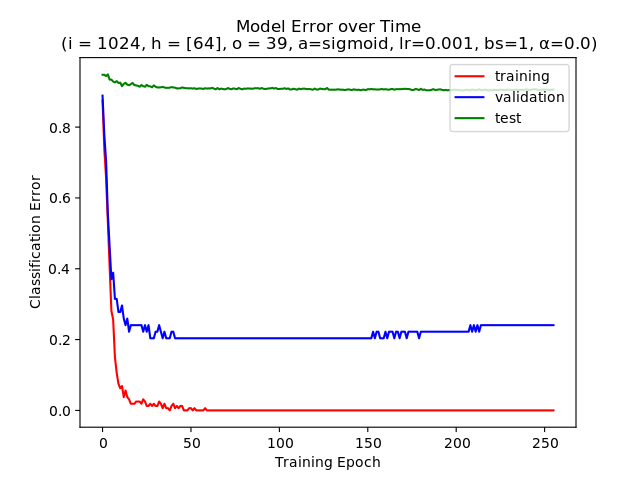
\includegraphics[width=0.5\textwidth]{./img/64-0.001-1-0-sigmoid-1/error-255.png}
      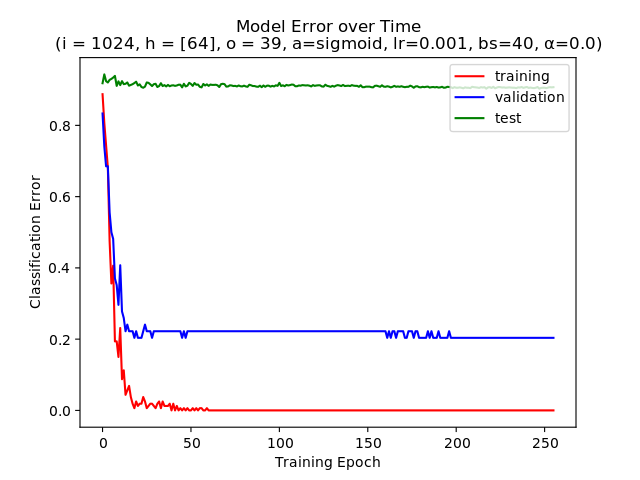
\includegraphics[width=0.5\textwidth]{./img/64-0.001-40-0-sigmoid-1/error-255.png}
      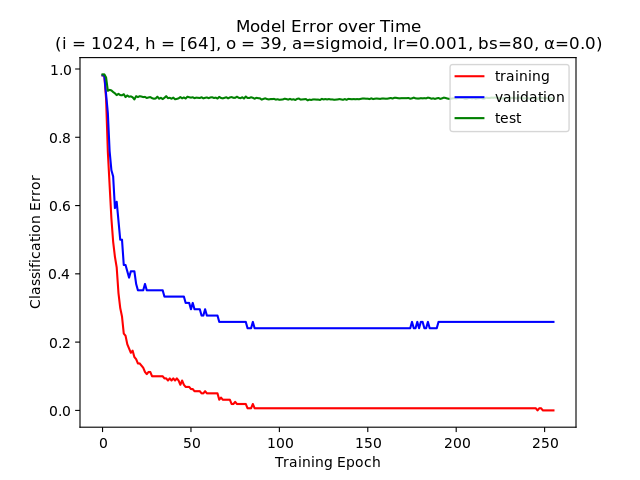
\includegraphics[width=0.5\textwidth]{./img/64-0.001-80-0-sigmoid-1/error-255.png}
      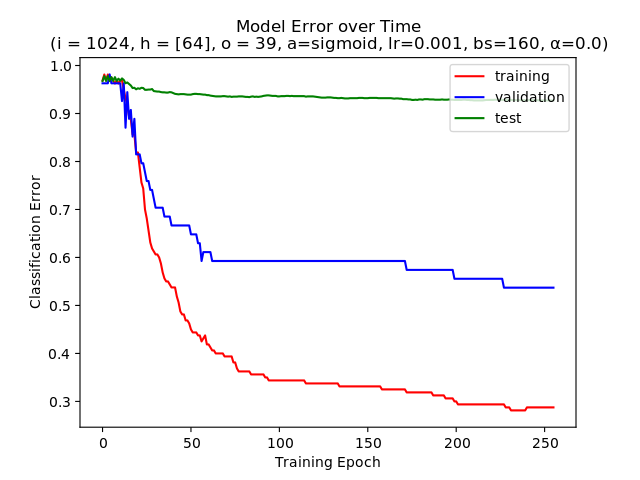
\includegraphics[width=0.5\textwidth]{./img/64-0.001-160-0-sigmoid-1/error-255.png}
      \caption{Classification Errors Varied by Batch Size}
      \label{fig:error-by-b}
    \end{figure}
    \paragraph{Variation in $N_H$}{
      Fig~\ref{fig:error-by-nh} illustrates the variation in accuracy resulting from a change in
      node count for the hidden layer. The lower, less expressive node counts appear to
      introduce significant jitter in the evolution of the error metric. This makes intuitive
      sense since a weight change in a single node has a greater potential impact on the hidden
      layer output when the nodes are few. There are fewer counterweights to counteract the mistakes
      of one hidden node. The lower count cases also reach the overfitting point much more quickly.
      There appears to be a linear relationship between the inflection point and the number of
      nodes. Assume a function $f$ that maps node count to the inflection epoch, i.e.,
      $f(N_H) = t_{overfit}$.
      In these examples, $f(1) \approx 75, f(4) \approx 100, f(16) \approx 175, f(64) > 256$.
    }
    \begin{figure}[h]
      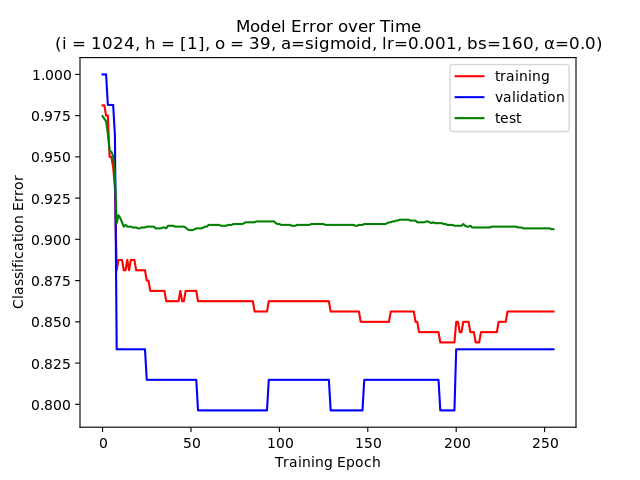
\includegraphics[width=0.5\textwidth]{./img/1-0.001-160-0-sigmoid-1/error-255.png}
      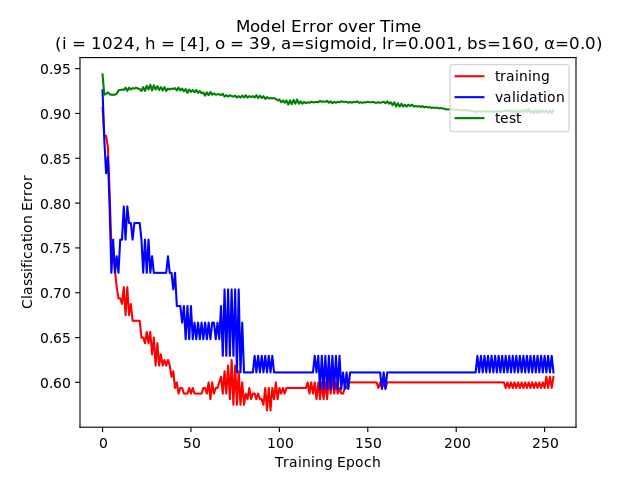
\includegraphics[width=0.5\textwidth]{./img/4-0.001-160-0-sigmoid-1/error-255.png}
      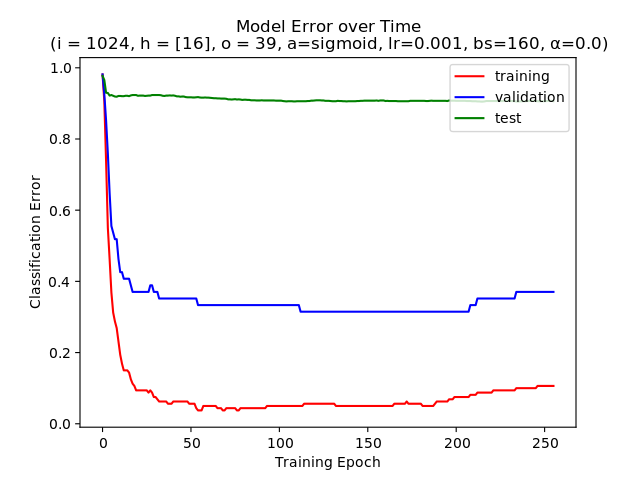
\includegraphics[width=0.5\textwidth]{./img/16-0.001-160-0-sigmoid-1/error-255.png}
      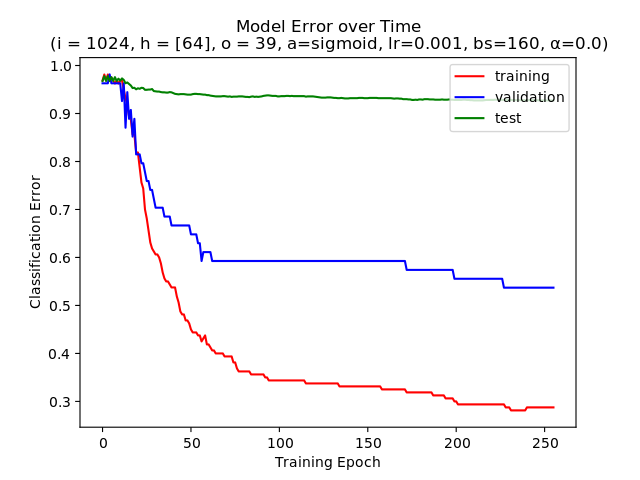
\includegraphics[width=0.5\textwidth]{./img/64-0.001-160-0-sigmoid-1/error-255.png}
      \caption{Classification Errors Varied by Hidden Layer Node Count}
      \label{fig:error-by-nh}
    \end{figure}
    %% \paragraph{Variation in $\alpha$}{
  }
  \subsection{Changes in Weight Over Time}{
    To plot changes in layer weights over the training cycle, a heatmap was adopted to simultaneously
    illustrate the changes for all layers in a single concise graphic. A consistent observation was
    that the weight changes quickly rose in a crescendo in the first few epochs of training and then
    quickly dropped off and stabilized. The classification error follows a similar enough pattern that
    the error graph might appear proportional to a cross-section of the weight change heat map
    if it were extruded into three-dimensional space. Plots for weight vector norm difference per epoch
    were created, but they are omitted here as the information is redundant with the angle delta plots.
    \paragraph{Variation in $b$}{
      Fig~\ref{fig:dw-by-b} illustrates the weight change history for variations in batch size.
      As batch size increases, the weight changes become more gradual and less pronounced. This follows
      intuitively since smaller batch sizes incur opportunities for more immediate backpropagation
      multiple times within an epoch. As such, the model changes to fit each sample, becoming quicker
      to overfit as the batch size decreases.
    }
    \begin{figure}[h]
      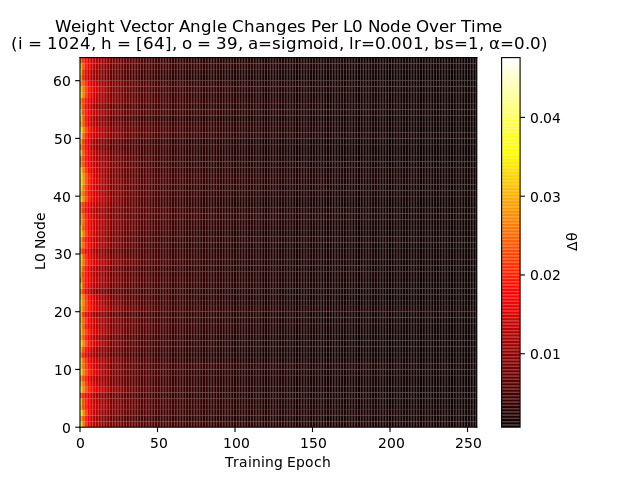
\includegraphics[width=0.5\textwidth]{./img/64-0.001-1-0-sigmoid-1/weight-angle-changes-L0-255.png}
      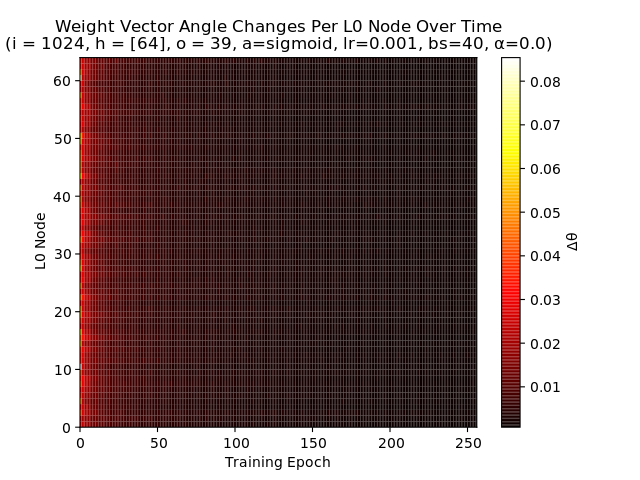
\includegraphics[width=0.5\textwidth]{./img/64-0.001-40-0-sigmoid-1/weight-angle-changes-L0-255.png}
      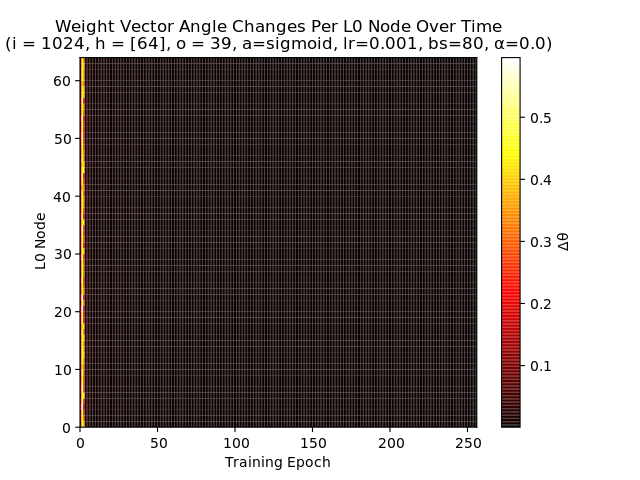
\includegraphics[width=0.5\textwidth]{./img/64-0.001-80-0-sigmoid-1/weight-angle-changes-L0-255.png}
      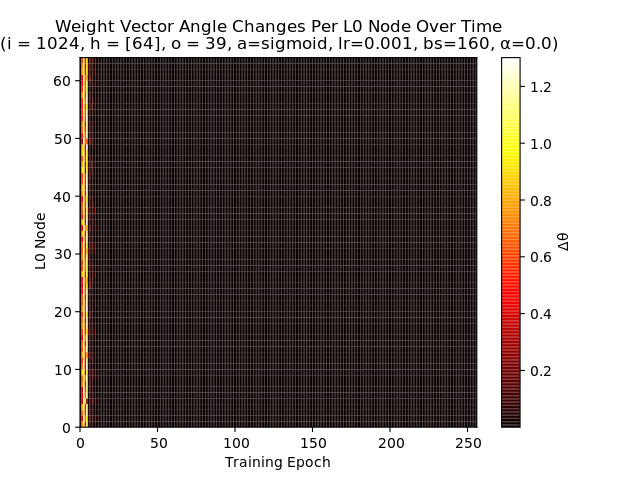
\includegraphics[width=0.5\textwidth]{./img/64-0.001-160-0-sigmoid-1/weight-angle-changes-L0-255.png}
      \caption{Activations Varied by Batch Size}
      \label{fig:dw-by-b}
    \end{figure}
    \paragraph{Variation in $N_H$}{
      Fig~\ref{fig:dw-by-nh} illustrates the weight change history for variations in hidden node count.
      With a single hidden node, the weight changes appear relatively small for the most part, although
      some of that may be an issue with artifacting in matplotlib that is masking the ostensible maxima.
      With four hidden nodes, it appears that nodes 0 and 2 incur the most sustained change over time,
      while nodes 1 and 3 remain relatively quiescent. As node count increases, the majority of the time
      is spent making minor adjustments with a burst of change in the early epochs. The burst is more
      pronounced in the $N_H = 64$ both in relative and absolute magnitude.
    }
    \begin{figure}[h]
      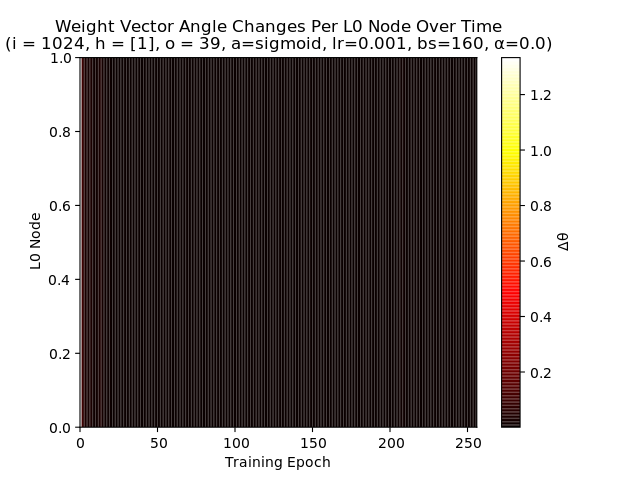
\includegraphics[width=0.5\textwidth]{./img/1-0.001-160-0-sigmoid-1/weight-angle-changes-L0-255.png}
      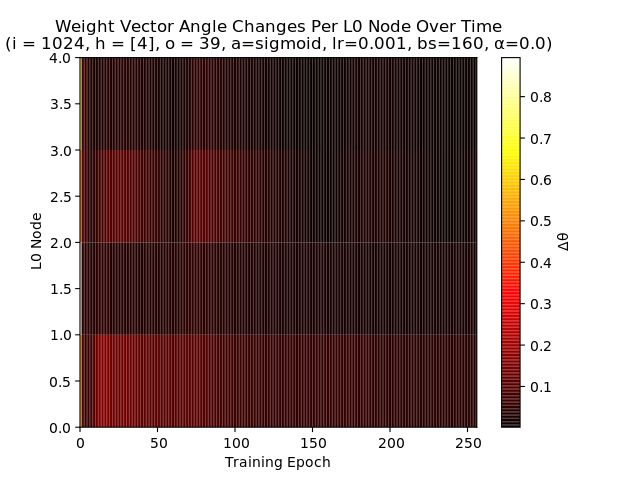
\includegraphics[width=0.5\textwidth]{./img/4-0.001-160-0-sigmoid-1/weight-angle-changes-L0-255.png}
      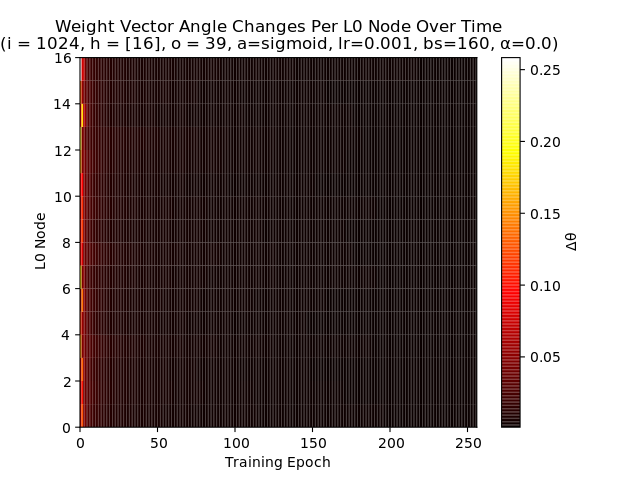
\includegraphics[width=0.5\textwidth]{./img/16-0.001-160-0-sigmoid-1/weight-angle-changes-L0-255.png}
      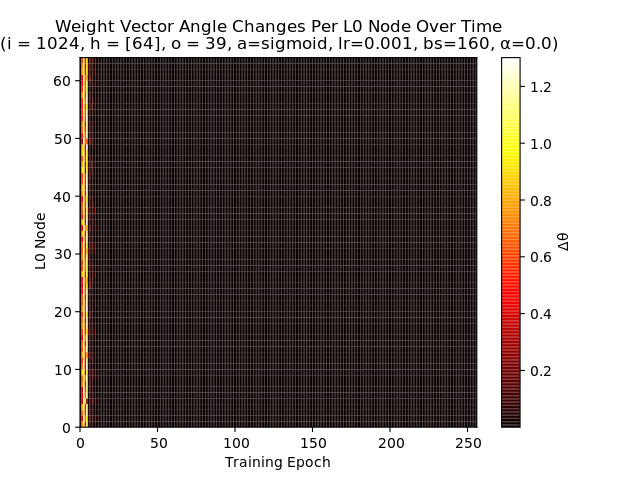
\includegraphics[width=0.5\textwidth]{./img/64-0.001-160-0-sigmoid-1/weight-angle-changes-L0-255.png}
      \caption{Weight Vector Changes Varied by Hidden Layer Node Count}
      \label{fig:dw-by-nh}
    \end{figure}
  }

  \subsection{Non-Linear Activations}{
    \paragraph{Variation in $b$}{
      Fig~\ref{fig:a-by-b} illustrates the output of the activation unit for each hidden input node
      over variations in batch size. When batch size is small, the distribution of activations
      appears to follow a normal distribution with mean at 0.5. As batch size increases, this
      gradually morphs into a bimodal distribution with peaks at 0 and 1. The distribution
      appear to be consistent across multiple nodes. The larger peak occurs around zero (0),
      which makes sense since the model is likely concentrating its ``voting power'' in the
      learned class outputs and zeroing out most others.
    }
    \begin{figure}[h]
      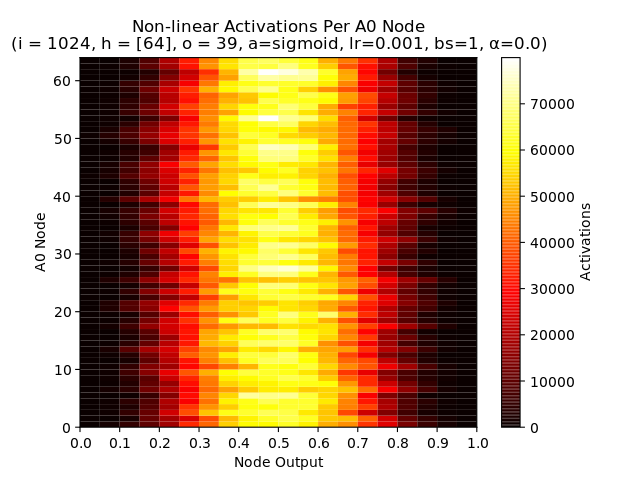
\includegraphics[width=0.5\textwidth]{./img/64-0.001-1-0-sigmoid-1/activations-A0-255.png}
      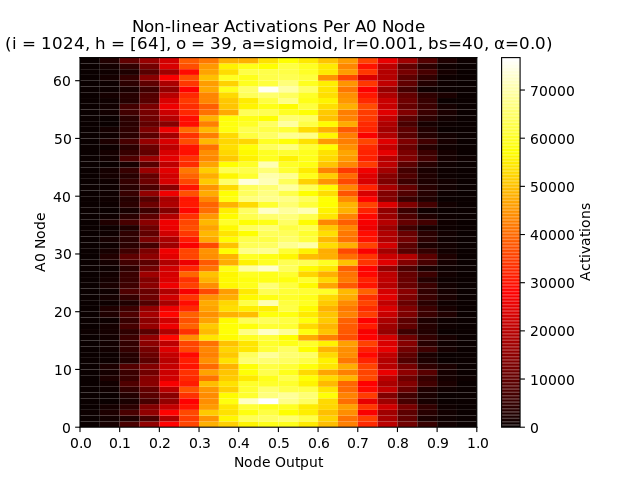
\includegraphics[width=0.5\textwidth]{./img/64-0.001-40-0-sigmoid-1/activations-A0-255.png}
      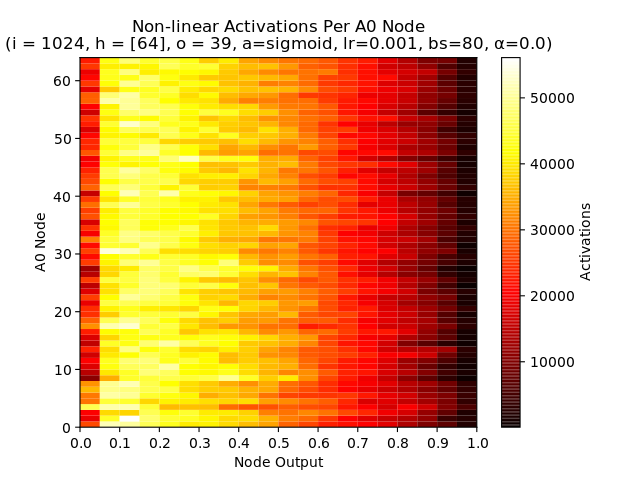
\includegraphics[width=0.5\textwidth]{./img/64-0.001-80-0-sigmoid-1/activations-A0-255.png}
      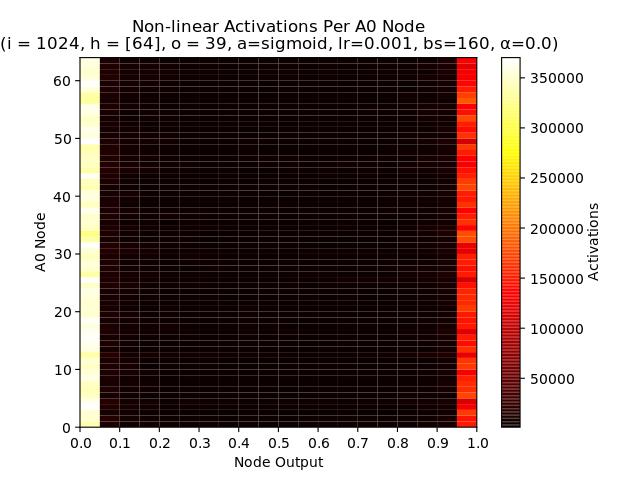
\includegraphics[width=0.5\textwidth]{./img/64-0.001-160-0-sigmoid-1/activations-A0-255.png}
      \caption{Activations Varied by Batch Size}
      \label{fig:a-by-b}
    \end{figure}
    \paragraph{Variation in $N_H$}{
      Fig~\ref{fig:a-by-nh} illustrates the output of the activation unit for each hidden input node
      over variations in hidden node count. The extrema in node count exhibit the bimodal distribution
      seen previously in the large batch size while the middle counts are closer to the normal
      distribution. The case where $N_H = 4$ appears to be more disorganized in its distribution
      than where $N_H = 16$, though this appears to correlate to the weight vector changes observed.

      This suggests that a node subject to more emphatic swings in its weights over longer periods of
      time will reflect this in the form of a normal random activation pattern, while nodes which remain
      relatively cool will settle into a stable bimodal pattern. This may also correlate with
      the overfitting inflection point, which does not appear to be reached in the case where $N_H = 64$.

      It should be noted that the $N_H = 1$, while bimodal, has a more gradual slope than $N_H = 64$.
      This supports the prior supposition that extended jitter diffuses the activations over a wider
      area. The single node case may also be exhibiting some degeneracy by virtue of it having to compress
      a 39-class decision into a single scalar that is then weighted accordingly by the output layer.
    }
    \begin{figure}[h]
      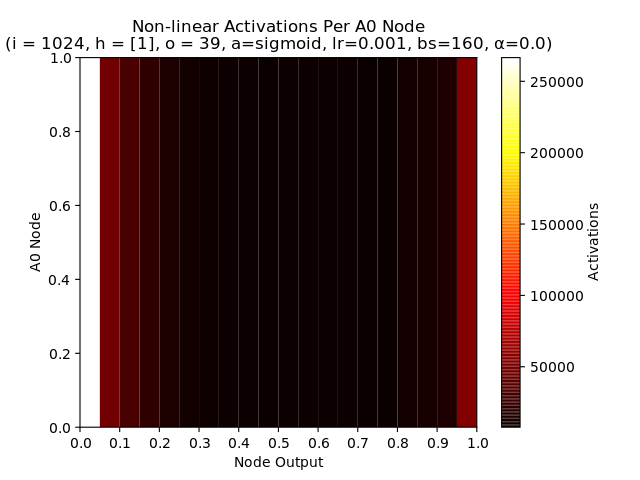
\includegraphics[width=0.5\textwidth]{./img/1-0.001-160-0-sigmoid-1/activations-A0-255.png}
      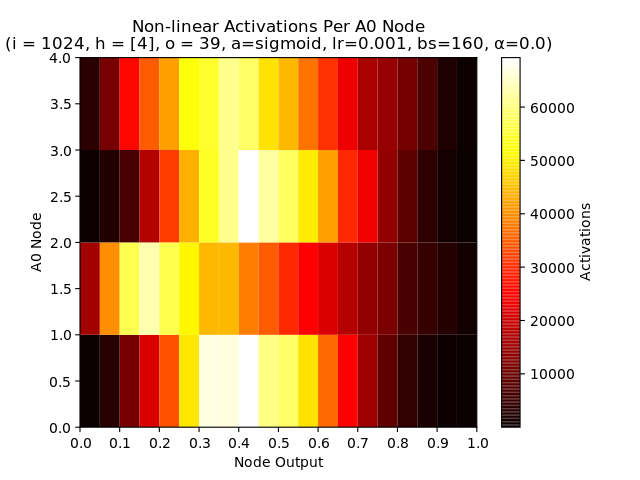
\includegraphics[width=0.5\textwidth]{./img/4-0.001-160-0-sigmoid-1/activations-A0-255.png}
      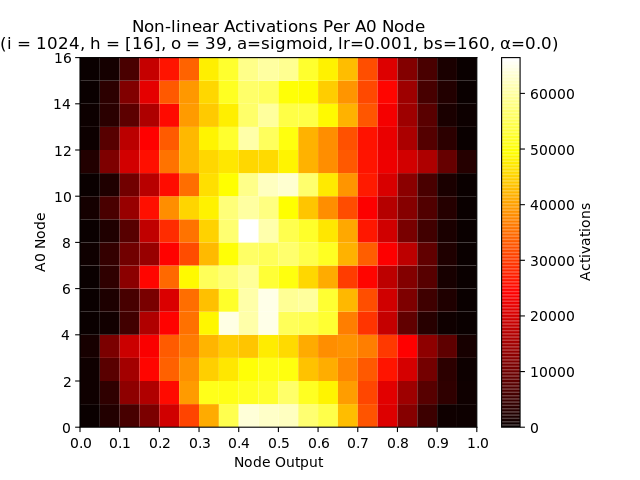
\includegraphics[width=0.5\textwidth]{./img/16-0.001-160-0-sigmoid-1/activations-A0-255.png}
      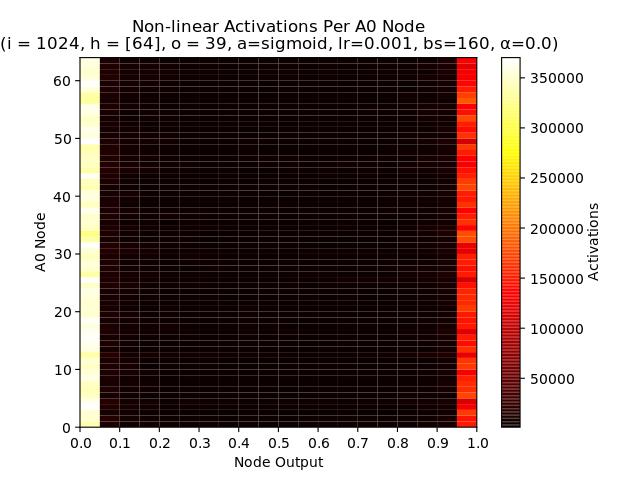
\includegraphics[width=0.5\textwidth]{./img/64-0.001-160-0-sigmoid-1/activations-A0-255.png}
      \caption{Activations Varied by Hidden Layer Node Count}
      \label{fig:a-by-nh}
    \end{figure}
  }
}
\section{Conclusions}{
}

\printbibliography
\end{document}
